%!TEX root = ../../../../memoria.tex
\subsection{Resumen de la compra}\label{chapter:solucionimplementada:checkout:review}

	Esta sección muestra un resumen de la compra que se esta realizando (ver \refFigura{figure:review:checkout:summary}). Esta información es parte del detalle completo que debe mostrar esta sección para dejar claro al cliente que es exactamente lo que esta comprando. Esto debe ser mejorado como trabajo futuro.

	\begin{figure}[!h]
		\centering
		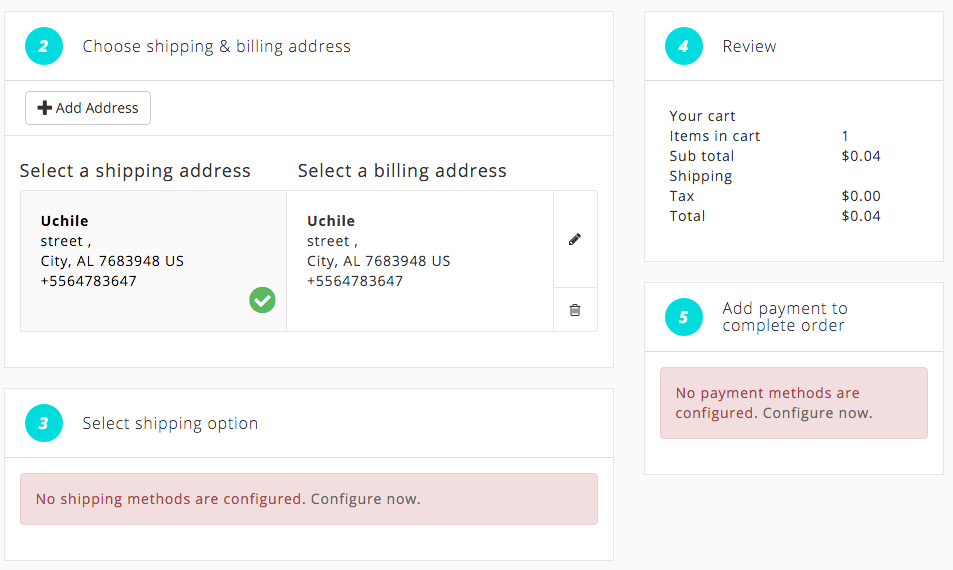
\includegraphics[width=0.8\textwidth]{figuras/shipping/steps.png}
		\caption{Detalle de la compra dentro del proceso de \checkoutEF.}
		\label{figure:review:checkout:summary}
	\end{figure}